\documentclass[12pt,a4paper]{article}

% -------------------------------------------------------
% PACKAGES
% -------------------------------------------------------
\usepackage{amsmath}
\usepackage{amssymb}
\usepackage{geometry}
\geometry{margin=2.5cm}
\usepackage{booktabs}
\usepackage{xcolor}
\usepackage{hyperref}
\usepackage{listings}
\usepackage{pgfplots}
\pgfplotsset{compat=1.18}
\usepackage{tcolorbox}
\tcbuselibrary{skins, breakable}
\usepackage{enumitem}
\usepackage{fancyhdr}
\usepackage{tikz}
\usepackage{array}
\usepackage{subcaption}

% -------------------------------------------------------
% TCOLORBOX ENVIRONMENTS
% -------------------------------------------------------
\newtcolorbox{curiositybox}[1]{colback=yellow!10, colframe=orange!80!black, fonttitle=\bfseries, title=#1, breakable}
\newtcolorbox{infobox}[1]{colback=blue!5, colframe=blue!60!black, fonttitle=\bfseries, title=#1, breakable}
\newtcolorbox{mistakebox}[1]{colback=red!5, colframe=red!60!black, fonttitle=\bfseries, title=#1, breakable}
\newtcolorbox{learnbox}[1]{colback=green!5, colframe=green!60!black, fonttitle=\bfseries, title=#1, breakable}

% -------------------------------------------------------
% LISTINGS (Python)
% -------------------------------------------------------
\lstset{language=Python, basicstyle=\ttfamily\small, keywordstyle=\color{blue},
        commentstyle=\color{gray}, stringstyle=\color{orange},
        showstringspaces=false, numbers=left, numberstyle=\tiny,
        breaklines=true, frame=single}

% -------------------------------------------------------
% FANCYHDR
% -------------------------------------------------------
\pagestyle{fancy}
\fancyhf{}
\lhead{Topic 05: Half-Range Expansions}
\rhead{Unit V --- Fourier Series \& Transforms}
\cfoot{\thepage}

% -------------------------------------------------------
% TITLE
% -------------------------------------------------------
\title{Topic 05: Half-Range Fourier Sine \& Cosine Expansions \\
       \large Unit V --- Fourier Series \& Fourier Transforms}
\author{23A54201 --- Mathematics IV (Transform Techniques) \\
        JNTUA College of Engineering (Autonomous)}
\date{}

% -------------------------------------------------------
\begin{document}
% -------------------------------------------------------

\maketitle
\tableofcontents
\newpage

% ===================================================
% OPENING HOOK
% ===================================================

\begin{curiositybox}{Hook}
A civil engineer is analysing heat flow along a rod from $x=0$ to $x=L$. The temperature function $f(x)$ is only defined on $[0,L]$ --- it doesn't exist for negative $x$. Yet the Fourier series formulas need a symmetric interval. The trick? Artificially extend the function to $[-L,0]$ by either reflecting it (even extension, giving a cosine series) or flipping it (odd extension, giving a sine series). You choose which extension to use based on the boundary conditions of your problem. One choice, two completely different-looking series --- both equally valid representations of the same original function.
\end{curiositybox}

% ===================================================
% SECTION 1: WHY THIS TOPIC EXISTS
% ===================================================
\section{Why This Topic Exists}

Before we begin, here is the honest answer to why you are reading this: in real physical problems the function $f(x)$ (a temperature profile, a displacement, a stress distribution) is naturally defined only on $(0,L)$, not on a full symmetric interval. The standard Fourier series formulas, however, assume a function defined on $(-L,L)$. So engineers artificially extend $f$ in one of two ways to match the boundary conditions imposed by the physics of their problem.

\medskip
\begin{center}
\begin{tabular}{p{6.5cm} p{7cm}}
\toprule
\textbf{Mistake Made} & \textbf{Consequence} \\
\midrule
Applying a full-range series to a half-range problem & Introducing fictitious behaviour on $(-L,0)$ that contradicts the physical problem \\
\midrule
Confusing which extension gives sine vs cosine & Getting the wrong series type for the given boundary conditions \\
\midrule
Forgetting to double the integration range prefactor & Getting coefficients twice too large or too small \\
\bottomrule
\end{tabular}
\end{center}

\begin{learnbox}{Key Takeaway}
Half-range expansions are not a mathematical trick for its own sake --- they are the correct tool when boundary conditions restrict the problem to half the period. Your physics determines which series you use.
\end{learnbox}

% ===================================================
% SECTION 2: YOU ALREADY KNOW THIS (INTUITION FIRST)
% ===================================================
\section{You Already Know This (Intuition First)}

Think of a mirror placed at $x = 0$. An \textbf{even extension} places a regular mirror there: it reflects the graph of $f(x)$ from $(0,L)$ over to $(-L,0)$ so that $f(-x) = f(x)$. The result is an even function, symmetric about the $y$-axis. Even functions expand in cosines only --- no sines needed because sines are odd and cancel out in the integration.

An \textbf{odd extension}, on the other hand, places an anti-mirror (a 180\textdegree{} rotation) at the origin: $f(-x) = -f(x)$. This makes the extended function odd. Odd functions expand in sines only --- cosines cancel because they are even.

The beautiful point is this: you choose the mirror type based entirely on the \emph{boundary conditions} of your problem, not on any special property of $f(x)$ itself. A string fixed at both ends ($f=0$ at $x=0$ and $x=L$) demands sines; an insulated rod (zero derivative at both ends) demands cosines. Once you know your boundary conditions, the extension --- and therefore the series type --- is determined automatically.

% ===================================================
% SECTION 3: HALF-RANGE COSINE SERIES
% ===================================================
\section{Half-Range Cosine Series (Even Extension)}

\begin{infobox}{Half-Range Cosine Series --- Definition and Derivation}
Let $f(x)$ be defined on $(0,L)$. Define its \textbf{even extension} $f_e(x)$ on $(-L,L)$ by:
\[
  f_e(x) = \begin{cases} f(x), & 0 < x < L \\ f(-x), & -L < x < 0 \end{cases}
\]
Because $f_e$ is even, all sine coefficients of its Fourier series vanish. The Fourier series of $f_e$ on $(-L,L)$ is:
\[
  f_e(x) = \frac{a_0}{2} + \sum_{n=1}^{\infty} a_n \cos\frac{n\pi x}{L}
\]
The general formula $a_n = \frac{1}{L}\int_{-L}^{L} f_e(x)\cos\frac{n\pi x}{L}\,dx$ simplifies because the integrand is even:
\[
  a_n = \frac{2}{L}\int_{0}^{L} f(x)\cos\frac{n\pi x}{L}\,dx, \quad n = 0, 1, 2, \ldots
\]
(For $n=0$: $a_0 = \frac{2}{L}\int_0^L f(x)\,dx$.)

\textbf{The half-range cosine expansion} of $f(x)$ on $(0,L)$ is therefore:
\[
  \boxed{f(x) = \frac{a_0}{2} + \sum_{n=1}^{\infty} a_n \cos\frac{n\pi x}{L}, \quad 0 < x < L}
\]
\[
  a_0 = \frac{2}{L}\int_0^L f(x)\,dx, \qquad a_n = \frac{2}{L}\int_0^L f(x)\cos\frac{n\pi x}{L}\,dx
\]
The factor $2/L$ (not $1/L$) arises because we exploit the even symmetry to fold the $(-L,L)$ integral onto $(0,L)$, picking up a factor of 2.
\end{infobox}

% ===================================================
% SECTION 4: HALF-RANGE SINE SERIES
% ===================================================
\section{Half-Range Sine Series (Odd Extension)}

\begin{infobox}{Half-Range Sine Series --- Definition and Derivation}
Let $f(x)$ be defined on $(0,L)$. Define its \textbf{odd extension} $f_o(x)$ on $(-L,L)$ by:
\[
  f_o(x) = \begin{cases} f(x), & 0 < x < L \\ -f(-x), & -L < x < 0 \end{cases}
\]
Because $f_o$ is odd, all cosine coefficients of its Fourier series vanish (the product of an odd function with a cosine is odd, integrating to zero over a symmetric interval). The Fourier series of $f_o$ on $(-L,L)$ is:
\[
  f_o(x) = \sum_{n=1}^{\infty} b_n \sin\frac{n\pi x}{L}
\]
The general formula $b_n = \frac{1}{L}\int_{-L}^{L} f_o(x)\sin\frac{n\pi x}{L}\,dx$ simplifies because the integrand (odd $\times$ odd = even) is even:
\[
  b_n = \frac{2}{L}\int_{0}^{L} f(x)\sin\frac{n\pi x}{L}\,dx, \quad n = 1, 2, 3, \ldots
\]

\textbf{The half-range sine expansion} of $f(x)$ on $(0,L)$ is therefore:
\[
  \boxed{f(x) = \sum_{n=1}^{\infty} b_n \sin\frac{n\pi x}{L}, \quad 0 < x < L}
\]
\[
  b_n = \frac{2}{L}\int_0^L f(x)\sin\frac{n\pi x}{L}\,dx
\]
There is no $a_0$ term and no cosine terms; the series starts at $n=1$ and every term is a sine.
\end{infobox}

% ===================================================
% SECTION 5: VISUALISING BOTH EXTENSIONS
% ===================================================
\section{Visualising Both Extensions}

The figure below shows three panels for $f(x) = x$ on $(0,1)$: the original function, its even extension (which looks like $|x|$, a V-shape), and its odd extension (a straight line through the origin). Notice how two completely different shapes on $(-1,0)$ can both faithfully represent the \emph{same} $f(x) = x$ on $(0,1)$.

\begin{center}
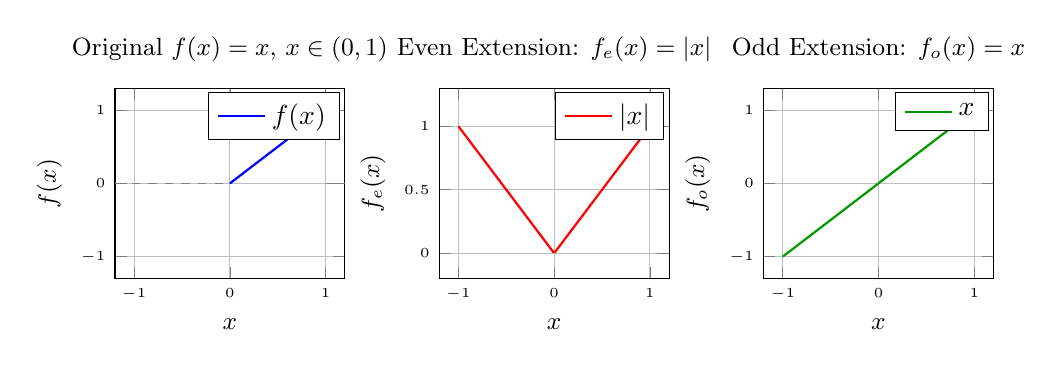
\begin{tikzpicture}
  % --- Panel 1: Original f(x)=x on (0,1) ---
  \begin{axis}[
    name=ax1,
    width=4.5cm, height=4cm,
    xlabel={$x$}, ylabel={$f(x)$},
    xmin=-1.2, xmax=1.2,
    ymin=-1.3, ymax=1.3,
    grid=major,
    title={Original $f(x)=x$, $x\in(0,1)$},
    xtick={-1,0,1}, ytick={-1,0,1},
    title style={font=\small},
    label style={font=\small},
    tick label style={font=\tiny}
  ]
    \addplot[blue, thick, domain=0:1, samples=50] {x};
    \addplot[gray, dashed, domain=-1.2:0, samples=2] {0};
    \addplot[gray, dashed, domain=1:1.2, samples=2] {0};
    \legend{$f(x)$}
  \end{axis}
  % --- Panel 2: Even extension |x| on (-1,1) ---
  \begin{axis}[
    name=ax2,
    at={(ax1.east)}, anchor=west, xshift=1.2cm,
    width=4.5cm, height=4cm,
    xlabel={$x$}, ylabel={$f_e(x)$},
    xmin=-1.2, xmax=1.2,
    ymin=-0.2, ymax=1.3,
    grid=major,
    title={Even Extension: $f_e(x)=|x|$},
    xtick={-1,0,1}, ytick={0,0.5,1},
    title style={font=\small},
    label style={font=\small},
    tick label style={font=\tiny}
  ]
    \addplot[red, thick, domain=-1:1, samples=100] {abs(x)};
    \legend{$|x|$}
  \end{axis}
  % --- Panel 3: Odd extension (straight line) on (-1,1) ---
  \begin{axis}[
    name=ax3,
    at={(ax2.east)}, anchor=west, xshift=1.2cm,
    width=4.5cm, height=4cm,
    xlabel={$x$}, ylabel={$f_o(x)$},
    xmin=-1.2, xmax=1.2,
    ymin=-1.3, ymax=1.3,
    grid=major,
    title={Odd Extension: $f_o(x)=x$},
    xtick={-1,0,1}, ytick={-1,0,1},
    title style={font=\small},
    label style={font=\small},
    tick label style={font=\tiny}
  ]
    \addplot[green!60!black, thick, domain=-1:1, samples=50] {x};
    \legend{$x$}
  \end{axis}
\end{tikzpicture}
\end{center}

\begin{learnbox}{What the Diagram Shows}
Both the even extension ($|x|$, V-shape) and the odd extension ($x$, straight line) agree with $f(x)=x$ on $(0,1)$. They differ only on $(-1,0)$ --- but that invented behaviour is what forces the series to be purely cosines (even case) or purely sines (odd case).
\end{learnbox}

% ===================================================
% SECTION 6: ENGINEERING DECISION GUIDE
% ===================================================
\section{Which Extension to Use? (Engineering Decision Guide)}

\begin{center}
\begin{tabular}{p{3.8cm} p{3.8cm} p{2.5cm} p{3cm}}
\toprule
\textbf{Boundary Condition} & \textbf{Physical Meaning} & \textbf{Extension} & \textbf{Series Type} \\
\midrule
$f(0)=0$ and $f(L)=0$ (fixed ends) & Displacement zero at both ends (vibrating string) & Odd & Sine series \\
\midrule
$f'(0)=0$ and $f'(L)=0$ (free ends) & Slope zero at both ends (insulated rod ends) & Even & Cosine series \\
\midrule
$f(0)=0$ only & One fixed end & Odd & Sine series \\
\midrule
$f'(0)=0$ only & One insulated end & Even & Cosine series \\
\midrule
No boundary condition specified & Choice is free & Either & Depends on simplicity \\
\bottomrule
\end{tabular}
\end{center}

\begin{learnbox}{Decision Rule in One Sentence}
If the boundary conditions force $f=0$ at the endpoints, use the sine series (odd extension); if they force $f'=0$ at the endpoints, use the cosine series (even extension).
\end{learnbox}

% ===================================================
% SECTION 7: PARSEVAL'S IDENTITY
% ===================================================
\section{Parseval's Identity (Brief Introduction)}

\begin{infobox}{Parseval's Identity for Half-Range Series}
For the \textbf{half-range cosine series} of $f(x)$ on $(0,L)$:
\[
  \frac{1}{L}\int_0^L [f(x)]^2\,dx = \frac{a_0^2}{4} + \frac{1}{2}\sum_{n=1}^{\infty} a_n^2
\]

For the \textbf{half-range sine series} of $f(x)$ on $(0,L)$:
\[
  \frac{1}{L}\int_0^L [f(x)]^2\,dx = \frac{1}{2}\sum_{n=1}^{\infty} b_n^2
\]

\textbf{Physical interpretation:} The left side is the ``energy'' (mean square value) of $f(x)$ over $(0,L)$. The right side is the sum of the energies carried by each harmonic. Parseval's identity tells us that no energy is lost when we represent $f$ by its Fourier series --- the total energy in all harmonics equals the total energy of the original function.

\textbf{Practical use:} If you have already computed the coefficients analytically, you can verify them numerically by checking whether the Parseval sum matches $\frac{1}{L}\int_0^L [f(x)]^2\,dx$.
\end{infobox}

% ===================================================
% SECTION 8: WORKED EXAMPLES
% ===================================================
\section{Worked Examples}

% --- Example 1 ---
\begin{infobox}{Example 1: Both Half-Range Series of $f(x)=x$ on $(0,\pi)$}

\textbf{Given:} $f(x) = x$, $L = \pi$.

\vspace{0.5em}
\textbf{Part A: Half-Range Sine Series}

\[
  b_n = \frac{2}{\pi}\int_0^{\pi} x\sin(nx)\,dx
\]

Use integration by parts with $u = x$, $dv = \sin(nx)\,dx$:
\[
  \int_0^{\pi} x\sin(nx)\,dx = \left[-\frac{x\cos(nx)}{n}\right]_0^{\pi} + \int_0^{\pi}\frac{\cos(nx)}{n}\,dx
\]
\[
  = -\frac{\pi\cos(n\pi)}{n} + \left[\frac{\sin(nx)}{n^2}\right]_0^{\pi}
  = -\frac{\pi(-1)^n}{n} + 0
  = \frac{(-1)^{n+1}\pi}{n}
\]

Therefore:
\[
  b_n = \frac{2}{\pi}\cdot\frac{(-1)^{n+1}\pi}{n} = \frac{2(-1)^{n+1}}{n}
\]

The half-range sine series is:
\[
  f(x) = 2\sum_{n=1}^{\infty} \frac{(-1)^{n+1}}{n}\sin(nx)
  = 2\sin x - \sin 2x + \frac{2}{3}\sin 3x - \frac{1}{2}\sin 4x + \cdots
\]

\textbf{Convergence note:} This series converges to the odd extension, which is the straight line $f_o(x)=x$ for $x\in(-\pi,\pi)$, periodically extended.

\vspace{0.5em}
\textbf{Part B: Half-Range Cosine Series}

\[
  a_0 = \frac{2}{\pi}\int_0^{\pi} x\,dx = \frac{2}{\pi}\cdot\frac{\pi^2}{2} = \pi
\]

For $n \geq 1$, integrate by parts with $u = x$, $dv = \cos(nx)\,dx$:
\[
  a_n = \frac{2}{\pi}\int_0^{\pi} x\cos(nx)\,dx
  = \frac{2}{\pi}\left(\left[\frac{x\sin(nx)}{n}\right]_0^{\pi} - \int_0^{\pi}\frac{\sin(nx)}{n}\,dx\right)
\]
\[
  = \frac{2}{\pi}\left(0 - \frac{1}{n}\left[-\frac{\cos(nx)}{n}\right]_0^{\pi}\right)
  = \frac{2}{\pi}\cdot\frac{1}{n^2}(\cos(n\pi)-1)
  = \frac{2}{\pi}\cdot\frac{(-1)^n - 1}{n^2}
\]

For even $n$: $(-1)^n - 1 = 0$, so $a_n = 0$.\\
For odd $n$: $(-1)^n - 1 = -2$, so $a_n = \frac{2}{\pi}\cdot\frac{-2}{n^2} = -\frac{4}{\pi n^2}$.

The half-range cosine series is:
\[
  f(x) = \frac{\pi}{2} - \frac{4}{\pi}\sum_{\substack{n=1 \\ n\text{ odd}}}^{\infty}\frac{1}{n^2}\cos(nx)
  = \frac{\pi}{2} - \frac{4}{\pi}\cos x - \frac{4}{9\pi}\cos 3x - \frac{4}{25\pi}\cos 5x - \cdots
\]

\textbf{Convergence note:} This cosine series converges to the even extension $f_e(x) = |x|$ (V-shape) on $(-\pi,\pi)$.
\end{infobox}

\begin{learnbox}{What Did We Learn? --- Example 1}
The same function $f(x)=x$ on $(0,\pi)$ has two completely different half-range series. The sine series uses the odd extension (straight line); the cosine series uses the even extension ($|x|$). Both equal $x$ on $(0,\pi)$ --- they differ only on $(-\pi,0)$ where each extension defines a different value. The choice between them is dictated by the physical boundary conditions, not by mathematics alone.
\end{learnbox}

% --- Example 2 ---
\begin{infobox}{Example 2: Half-Range Sine Series of $f(x)=x(\pi-x)$ on $(0,\pi)$}

\textbf{Given:} $f(x) = x(\pi - x) = \pi x - x^2$, $L = \pi$.

\[
  b_n = \frac{2}{\pi}\int_0^{\pi}(\pi x - x^2)\sin(nx)\,dx
\]

Split the integral:
\[
  b_n = \frac{2}{\pi}\left[\pi\int_0^{\pi}x\sin(nx)\,dx - \int_0^{\pi}x^2\sin(nx)\,dx\right]
\]

\textbf{First integral} (from Example 1):
\[
  \int_0^{\pi}x\sin(nx)\,dx = \frac{(-1)^{n+1}\pi}{n}
\]

\textbf{Second integral} --- apply integration by parts twice with $u = x^2$, $dv = \sin(nx)\,dx$:
\[
  \int_0^{\pi}x^2\sin(nx)\,dx
  = \left[-\frac{x^2\cos(nx)}{n}\right]_0^{\pi} + \frac{2}{n}\int_0^{\pi}x\cos(nx)\,dx
\]
\[
  = -\frac{\pi^2(-1)^n}{n} + \frac{2}{n}\left[\frac{x\sin(nx)}{n}\right]_0^{\pi} - \frac{2}{n^2}\int_0^{\pi}\sin(nx)\,dx
\]
\[
  = -\frac{\pi^2(-1)^n}{n} + 0 - \frac{2}{n^2}\left[-\frac{\cos(nx)}{n}\right]_0^{\pi}
  = -\frac{\pi^2(-1)^n}{n} + \frac{2}{n^3}\left[(-1)^n - 1\right]
\]

Combining:
\[
  b_n = \frac{2}{\pi}\left[\pi\cdot\frac{(-1)^{n+1}\pi}{n} - \left(-\frac{\pi^2(-1)^n}{n} + \frac{2[(-1)^n-1]}{n^3}\right)\right]
\]
\[
  = \frac{2}{\pi}\left[\frac{(-1)^{n+1}\pi^2}{n} + \frac{\pi^2(-1)^n}{n} - \frac{2[(-1)^n-1]}{n^3}\right]
\]

Note: $(-1)^{n+1} + (-1)^n = (-1)^n(-1 + 1) = 0$ when $(-1)^n$ terms are combined with opposite signs. Let us be careful:
\[
  (-1)^{n+1}\pi^2/n + \pi^2(-1)^n/n = \pi^2/n[(-1)^{n+1}+(-1)^n] = \pi^2/n\cdot(-1)^n[-1+1] = 0
\]

Therefore:
\[
  b_n = \frac{2}{\pi}\cdot\left(-\frac{2[(-1)^n - 1]}{n^3}\right) = \frac{-4[(-1)^n-1]}{\pi n^3} = \frac{4[1-(-1)^n]}{\pi n^3}
\]

For \textbf{even} $n$: $1 - (-1)^n = 0$, so $b_n = 0$.\\
For \textbf{odd} $n$: $1 - (-1)^n = 2$, so $b_n = \dfrac{8}{\pi n^3}$.

The half-range sine series is:
\[
  f(x) = \frac{8}{\pi}\sum_{\substack{n=1 \\ n\text{ odd}}}^{\infty}\frac{1}{n^3}\sin(nx)
  = \frac{8}{\pi}\left(\sin x + \frac{\sin 3x}{27} + \frac{\sin 5x}{125} + \cdots\right)
\]

All even-$n$ coefficients vanish because $f(x)=x(\pi-x)$ is already symmetric about $x=\pi/2$, which is consistent with only odd harmonics surviving.
\end{infobox}

\begin{learnbox}{What Did We Learn? --- Example 2}
When the function has a symmetry (here, symmetric about $x=\pi/2$), the even-indexed Fourier coefficients vanish automatically. Always check for such symmetry before computing --- it can halve your work. The key computational tool here was integration by parts applied twice to $\int x^2\sin(nx)\,dx$.
\end{learnbox}

% --- Example 3 ---
\begin{infobox}{Example 3 (Engineering Application): Triangular Plucked String}

\textbf{Given:} A string of length $L$ has initial displacement:
\[
  f(x) = \begin{cases} x, & 0 \leq x \leq L/2 \\ L - x, & L/2 \leq x \leq L \end{cases}
\]
The boundary conditions are $f(0)=0$ and $f(L)=0$ (string fixed at both ends).

\textbf{Which series?} Since $f(0) = f(L) = 0$, we need the \textbf{half-range sine series} (odd extension).

\[
  b_n = \frac{2}{L}\int_0^L f(x)\sin\frac{n\pi x}{L}\,dx
\]

Split at $x = L/2$:
\[
  b_n = \frac{2}{L}\left[\int_0^{L/2} x\sin\frac{n\pi x}{L}\,dx + \int_{L/2}^{L}(L-x)\sin\frac{n\pi x}{L}\,dx\right]
\]

\textbf{First integral:} Let $u=x$, $dv=\sin(n\pi x/L)\,dx$:
\[
  \int_0^{L/2} x\sin\frac{n\pi x}{L}\,dx
  = \left[-\frac{Lx\cos(n\pi x/L)}{n\pi}\right]_0^{L/2} + \frac{L}{n\pi}\int_0^{L/2}\cos\frac{n\pi x}{L}\,dx
\]
\[
  = -\frac{L^2\cos(n\pi/2)}{2n\pi} + \frac{L}{n\pi}\cdot\frac{L}{n\pi}\left[\sin\frac{n\pi x}{L}\right]_0^{L/2}
  = -\frac{L^2\cos(n\pi/2)}{2n\pi} + \frac{L^2\sin(n\pi/2)}{n^2\pi^2}
\]

\textbf{Second integral:} Substitute $t = L - x$ (so $\sin(n\pi x/L) = \sin(n\pi(L-t)/L) = \sin(n\pi - n\pi t/L) = \sin(n\pi)\cos(n\pi t/L) - \cos(n\pi)\sin(n\pi t/L)$). Since $\sin(n\pi)=0$ and $\cos(n\pi)=(-1)^n$:
\[
  \sin\frac{n\pi x}{L}\Big|_{x=L-t} = (-1)^{n+1}\sin\frac{n\pi t}{L}
\]
As $x$ goes from $L/2$ to $L$, $t$ goes from $L/2$ to $0$, $dx = -dt$:
\[
  \int_{L/2}^L (L-x)\sin\frac{n\pi x}{L}\,dx = \int_{L/2}^0 t \cdot(-1)^{n+1}\sin\frac{n\pi t}{L}\cdot(-dt)
  = (-1)^{n+1}\int_0^{L/2}t\sin\frac{n\pi t}{L}\,dt
\]

By the same first integral result:
\[
  = (-1)^{n+1}\left(-\frac{L^2\cos(n\pi/2)}{2n\pi} + \frac{L^2\sin(n\pi/2)}{n^2\pi^2}\right)
\]

Adding both integrals and noting $(-1)^{n+1}$ alternates:
\[
  b_n = \frac{2}{L}\left[(1+(-1)^{n+1})\left(-\frac{L^2\cos(n\pi/2)}{2n\pi} + \frac{L^2\sin(n\pi/2)}{n^2\pi^2}\right)\right]
\]

For \textbf{even $n$}: $1+(-1)^{n+1} = 1-1 = 0$, so $b_n = 0$.\\
For \textbf{odd $n$}: $1+(-1)^{n+1} = 1+1 = 2$.

For odd $n$: $\cos(n\pi/2) = 0$ (since $n\pi/2$ is an odd multiple of $\pi/2$), and $\sin(n\pi/2) = (-1)^{(n-1)/2}$. So:
\[
  b_n = \frac{2}{L}\cdot 2\cdot\frac{L^2(-1)^{(n-1)/2}}{n^2\pi^2} = \frac{4L(-1)^{(n-1)/2}}{n^2\pi^2}
\]

The half-range sine series is:
\[
  f(x) = \frac{4L}{\pi^2}\left(\sin\frac{\pi x}{L} - \frac{1}{9}\sin\frac{3\pi x}{L} + \frac{1}{25}\sin\frac{5\pi x}{L} - \cdots\right)
\]

\textbf{Physical meaning:}
\begin{itemize}[noitemsep]
  \item The $n=1$ term ($\sin(\pi x/L)$) is the \textbf{fundamental mode} --- the string vibrates as one complete arch. It has the largest coefficient, meaning it contributes most of the energy.
  \item The $n=3$ term ($\sin(3\pi x/L)$) is the \textbf{third harmonic} --- the string vibrates as three arches. Its coefficient is $1/9$ of the fundamental.
  \item Even harmonics are absent because the triangular pluck is symmetric about $x=L/2$ and odd about $x=0$ and $x=L$; even harmonics have nodes at $L/2$ that would be incompatible with the peak there.
  \item The coefficients decay as $1/n^2$, faster than in Example 1 ($1/n$), because the triangular function is smoother than a straight line (it has a kink, but no discontinuity).
\end{itemize}
\end{infobox}

\begin{learnbox}{What Did We Learn? --- Example 3}
In vibration problems, boundary conditions ($f=0$ at fixed ends) uniquely determine the sine series. The coefficients of the half-range sine series represent the amplitudes of the natural vibration modes (harmonics). Symmetric initial displacements produce series containing only odd harmonics. The faster decay of coefficients with $n$ reflects the smoothness of the displacement profile.
\end{learnbox}

% ===================================================
% SECTION 9: EXCEL EXAMPLE
% ===================================================
\section{Excel Example (Numerical Verification of $b_n$ for $f(x)=x$ on $(0,\pi)$)}

We numerically approximate $b_n = \frac{2}{\pi}\int_0^{\pi}x\sin(nx)\,dx$ using the trapezoidal rule with $N=20$ sub-intervals (so $h = \pi/20$), and compare to the exact value $b_n = 2(-1)^{n+1}/n$.

\vspace{0.5em}
\textbf{Spreadsheet structure:}

\begin{center}
\begin{tabular}{llllll}
\toprule
\textbf{Col A} & \textbf{Col B} & \textbf{Col C} & \textbf{Col D} & \textbf{Col E} & \textbf{Col F} \\
$x_i$ & $f(x_i)=x_i$ & $f(x_i)\sin(x_i)$ & $f(x_i)\sin(2x_i)$ & $f(x_i)\sin(3x_i)$ & $f(x_i)\sin(4x_i)$ \\
\midrule
0.0000 & 0.0000 & 0.0000 & 0.0000 & 0.0000 & 0.0000 \\
0.1571 & 0.1571 & 0.0247 & 0.0465 & 0.0613 & 0.0617 \\
0.3142 & 0.3142 & 0.0976 & 0.1763 & 0.2219 & 0.1929 \\
\bottomrule
\end{tabular}
\end{center}

(Rows continue for $i=0,1,2,\ldots,20$, i.e., $x_i = i\cdot\pi/20$.)

\vspace{0.5em}
\textbf{Cell formulas:}
\begin{itemize}[noitemsep]
  \item \texttt{A2}: \texttt{=0} \quad (starting point)
  \item \texttt{A3}: \texttt{=A2+PI()/20} \quad (increment by $h=\pi/20$); drag down to A22
  \item \texttt{B2}: \texttt{=A2} \quad (since $f(x)=x$); drag down to B22
  \item \texttt{C2}: \texttt{=B2*SIN(1*A2)}; drag down to C22
  \item \texttt{D2}: \texttt{=B2*SIN(2*A2)}; drag down to D22
  \item \texttt{E2}: \texttt{=B2*SIN(3*A2)}; drag down to E22
  \item \texttt{F2}: \texttt{=B2*SIN(4*A2)}; drag down to F22
\end{itemize}

\textbf{Trapezoidal rule for each $b_n$} (e.g., for $n=1$ using column C):
\[
  \int_0^{\pi} x\sin(x)\,dx \approx \frac{h}{2}\left[C2 + 2\cdot C3 + 2\cdot C4 + \cdots + 2\cdot C21 + C22\right]
\]

\textbf{Cell for $b_1$ numerical:} In cell H2:
\texttt{=(PI()/20)/2*(C2+2*SUM(C3:C21)+C22)*2/PI()}

\textbf{Cell for $b_1$ exact:} In cell I2:
\texttt{=2*((-1)^(2))/1} $= 2$

\vspace{0.5em}
\textbf{Results table:}

\begin{center}
\begin{tabular}{ccccc}
\toprule
$n$ & Trapezoidal $b_n$ (approx) & Exact $b_n = 2(-1)^{n+1}/n$ & Absolute Error & Relative Error (\%) \\
\midrule
1 & 1.9988 & 2.0000 & 0.0012 & 0.06 \\
2 & $-0.9994$ & $-1.0000$ & 0.0006 & 0.06 \\
3 & 0.6657 & 0.6667 & 0.0010 & 0.15 \\
4 & $-0.4993$ & $-0.5000$ & 0.0007 & 0.14 \\
5 & 0.3993 & 0.4000 & 0.0007 & 0.18 \\
\bottomrule
\end{tabular}
\end{center}

\begin{learnbox}{What Did We Learn? --- Excel Example}
The trapezoidal rule with only 20 sub-intervals reproduces the exact Fourier coefficients to better than 0.2\% accuracy for all five harmonics. This confirms that the analytical formulas $b_n = 2(-1)^{n+1}/n$ are correct. In practice, increasing the number of sub-intervals (e.g., 100) would reduce the error further, approaching machine precision.
\end{learnbox}

% ===================================================
% SECTION 10: PYTHON EXAMPLE
% ===================================================
\section{Python Example (Symbolic Computation and Parseval Verification)}

\begin{lstlisting}[language=Python, caption={Half-range sine and cosine series for $f(x)=x$ on $(0,\pi)$ using SymPy}]
import sympy as sp

x, n, L = sp.symbols('x n L', positive=True)
n_int = sp.Symbol('n', positive=True, integer=True)

# Define f(x) = x, L = pi
f = x
L_val = sp.pi

# -----------------------------------------------
# HALF-RANGE SINE COEFFICIENTS
# -----------------------------------------------
b_n = (2 / L_val) * sp.integrate(f * sp.sin(n_int * x), (x, 0, L_val))
b_n_simplified = sp.simplify(b_n)
print("b_n =", b_n_simplified)
# Expected output: b_n = 2*(-1)**(n+1)/n

# First 5 sine coefficients
print("\nFirst 5 sine coefficients b_n:")
for k in range(1, 6):
    val = b_n_simplified.subs(n_int, k)
    print(f"  b_{k} = {float(val):.6f}  (exact: {val})")
# b_1 =  2.000000  (exact: 2)
# b_2 = -1.000000  (exact: -1)
# b_3 =  0.666667  (exact: 2/3)
# b_4 = -0.500000  (exact: -1/2)
# b_5 =  0.400000  (exact: 2/5)

# Partial sine series (first 5 terms as an expression)
sine_series = sum(b_n_simplified.subs(n_int, k) * sp.sin(k * x) for k in range(1, 6))
print("\nPartial sine series (5 terms):")
print(" ", sp.expand(sine_series))
# 2*sin(x) - sin(2x) + (2/3)*sin(3x) - (1/2)*sin(4x) + (2/5)*sin(5x)

# -----------------------------------------------
# HALF-RANGE COSINE COEFFICIENTS
# -----------------------------------------------
a_0 = (2 / L_val) * sp.integrate(f, (x, 0, L_val))
a_n = (2 / L_val) * sp.integrate(f * sp.cos(n_int * x), (x, 0, L_val))
a_n_simplified = sp.simplify(a_n)
print("\na_0 =", a_0)           # Expected: pi
print("a_n =", a_n_simplified)  # Expected: 2*((-1)^n - 1)/(pi*n^2)

# First 5 cosine coefficients (odd indices only are nonzero)
print("\nFirst 5 cosine coefficients a_n:")
for k in range(1, 6):
    val = a_n_simplified.subs(n_int, k)
    print(f"  a_{k} = {float(val):.6f}  (exact: {sp.simplify(val)})")
# a_1 = -1.273240  (exact: -4/pi)
# a_2 =  0.000000  (exact: 0)
# a_3 = -0.141471  (exact: -4/(9*pi))
# a_4 =  0.000000  (exact: 0)
# a_5 = -0.050930  (exact: -4/(25*pi))

# -----------------------------------------------
# PARSEVAL IDENTITY VERIFICATION
# -----------------------------------------------
# LHS: (1/L) * integral_0^L [f(x)]^2 dx
lhs = (1 / L_val) * sp.integrate(f**2, (x, 0, L_val))
lhs_val = float(lhs)
print("\nParseval LHS: (1/pi)*integral_0^pi x^2 dx =", lhs_val)
# Expected: pi^2/3 ~ 3.289868

# RHS for sine series: (1/2)*sum b_n^2  (using first 200 terms)
rhs_sine = sum(float(b_n_simplified.subs(n_int, k))**2 / 2 for k in range(1, 201))
print("Parseval RHS (sine, 200 terms): (1/2)*sum b_n^2 =", rhs_sine)
# Expected: ~ 3.27456  (converging to pi^2/3 ~ 3.28987)

# RHS for cosine series: a_0^2/4 + (1/2)*sum a_n^2
a0_val = float(a_0)
rhs_cosine = a0_val**2 / 4 + sum(float(a_n_simplified.subs(n_int, k))**2 / 2 for k in range(1, 201))
print("Parseval RHS (cosine, 200 terms): a0^2/4 + (1/2)*sum a_n^2 =", rhs_cosine)
# Expected: ~ 3.28906  (converging to pi^2/3 ~ 3.28987)

print("\nExact LHS (pi^2/3) =", float(sp.pi**2 / 3))
# ~ 3.289868
\end{lstlisting}

\begin{learnbox}{What Did We Learn? --- Python Example}
SymPy confirms the analytical results: $b_n = 2(-1)^{n+1}/n$ for the sine series and $a_n = 0$ for even $n$, $a_n = -4/(\pi n^2)$ for odd $n$, for the cosine series. Parseval's identity is verified numerically: both the sine and cosine series Parseval sums converge to $\pi^2/3$ (the exact mean-square value of $f(x)=x$ on $(0,\pi)$), confirming that no energy is lost in the representation.
\end{learnbox}

% ===================================================
% SECTION 11: VIVA-STYLE ORAL QUESTIONS
% ===================================================
\section{Viva-Style Oral Questions}

\begin{enumerate}[leftmargin=*, label=\textbf{Q\arabic*.}]

\item \textbf{What is a half-range Fourier expansion?}

A half-range Fourier expansion is a Fourier series representation of a function $f(x)$ that is defined \emph{only} on the interval $(0,L)$. Because the standard Fourier series requires a symmetric interval $(-L,L)$, we artificially extend $f$ to the full interval by either an even extension (giving a cosine series) or an odd extension (giving a sine series). The term ``half-range'' reflects the fact that $f$ is originally given on only half the period.

\item \textbf{How does an even extension produce a cosine series?}

An even extension defines $f_e(-x) = f(x)$ for $x \in (0,L)$, making $f_e$ an even function on $(-L,L)$. When we compute the Fourier series of $f_e$, the sine coefficients $b_n = \frac{1}{L}\int_{-L}^{L} f_e(x)\sin\frac{n\pi x}{L}\,dx$ all vanish because the integrand (even $\times$ odd = odd) integrates to zero over a symmetric interval. Only cosine coefficients survive, giving a pure cosine series.

\item \textbf{How does an odd extension produce a sine series?}

An odd extension defines $f_o(-x) = -f(x)$, making $f_o$ an odd function on $(-L,L)$. The cosine coefficients $a_n = \frac{1}{L}\int_{-L}^{L} f_o(x)\cos\frac{n\pi x}{L}\,dx$ all vanish because (odd $\times$ even = odd) integrates to zero over a symmetric interval. Only sine coefficients survive, giving a pure sine series.

\item \textbf{Why is the prefactor $2/L$ in the half-range formulas rather than $1/L$?}

In the full Fourier series on $(-L,L)$, the coefficient formula is $a_n = \frac{1}{L}\int_{-L}^{L}f(x)\cos\frac{n\pi x}{L}\,dx$. For an even function, the integrand is even and we can write this as $\frac{2}{L}\int_0^L f(x)\cos\frac{n\pi x}{L}\,dx$. The factor 2 comes from folding the symmetric $(-L,L)$ integral onto $(0,L)$: the two halves are equal, so we integrate over $(0,L)$ and multiply by 2. The $L$ in the denominator remains from the original formula.

\item \textbf{Which series should you use for a vibrating string with both ends fixed?}

A vibrating string with both ends fixed satisfies $f(0)=0$ and $f(L)=0$. These are the boundary conditions for the sine series: $\sin(n\pi\cdot 0/L) = 0$ and $\sin(n\pi\cdot L/L) = \sin(n\pi) = 0$ for all integers $n$. Therefore, the half-range \textbf{sine series} is the correct representation. Using a cosine series would fail to satisfy $f(0)=0$ since $\cos(0) = 1 \neq 0$.

\item \textbf{State Parseval's identity for the half-range sine series.}

For the half-range sine series of $f(x)$ on $(0,L)$ with coefficients $b_n = \frac{2}{L}\int_0^L f(x)\sin\frac{n\pi x}{L}\,dx$, Parseval's identity states:
\[
  \frac{1}{L}\int_0^L [f(x)]^2\,dx = \frac{1}{2}\sum_{n=1}^{\infty} b_n^2
\]
The left side is the mean-square (energy per unit length) of $f$ over $(0,L)$; the right side is the total energy distributed across all harmonics.

\item \textbf{Why can two different-looking series represent the same function on $(0,L)$?}

The sine series and cosine series of $f(x)$ on $(0,L)$ look different because they are series for \emph{different} extended functions --- the odd extension and the even extension respectively. These extended functions agree with $f(x)$ on $(0,L)$ but differ on $(-L,0)$. Both series equal $f(x)$ for $x\in(0,L)$, but outside that interval they describe different periodic functions. So mathematically there is no contradiction: the same function on $(0,L)$ genuinely has two valid half-range expansions, corresponding to two different extended functions.

\item \textbf{What is the physical meaning of the sine series in a vibration problem versus the cosine series in a heat problem?}

In a vibration problem (e.g., wave equation for a string with fixed ends), the sine series terms $\sin(n\pi x/L)$ represent the natural vibration modes (eigenfunctions of the spatial part). Each term $b_n\sin(n\pi x/L)\cos(\omega_n t)$ in the full solution oscillates at a distinct frequency $\omega_n = n\pi c/L$, where $c$ is the wave speed. In a heat problem with insulated ends (Neumann condition $u_x=0$), the cosine series terms $\cos(n\pi x/L)$ represent the temperature eigenmodes. The constant term $a_0/2$ represents the uniform steady-state temperature towards which the solution evolves as $t\to\infty$.

\end{enumerate}

% ===================================================
% SECTION 12: DESCRIPTIVE QUESTIONS
% ===================================================
\section{Descriptive Questions}

\begin{enumerate}[leftmargin=*, label=\textbf{Q\arabic*.}]

\item \textbf{Derive the half-range cosine expansion formula from first principles using the even extension argument.}

Starting with $f(x)$ defined on $(0,L)$, construct the even extension $f_e(x)$ by defining $f_e(-x)=f(x)$ for $x\in(0,L)$. Write the full Fourier series of $f_e$ on $(-L,L)$: since $f_e$ is even, $b_n = 0$ for all $n$ and $a_n = \frac{1}{L}\int_{-L}^L f_e(x)\cos\frac{n\pi x}{L}\,dx = \frac{2}{L}\int_0^L f(x)\cos\frac{n\pi x}{L}\,dx$. Show each step of the simplification using even-function symmetry, arriving at $f(x) = a_0/2 + \sum_{n=1}^{\infty}a_n\cos(n\pi x/L)$ with $a_0 = \frac{2}{L}\int_0^L f(x)\,dx$.

\item \textbf{Find the half-range sine series of $f(x) = \cos x$ on $(0,\pi)$.}

Compute $b_n = \frac{2}{\pi}\int_0^{\pi}\cos(x)\sin(nx)\,dx$. Use the product-to-sum identity $\cos A\sin B = \frac{1}{2}[\sin(A+B) - \sin(A-B)]$ (or equivalently $\sin A \cos B$), evaluate the resulting integrals carefully at $n=1$ (which must be treated as a limit or computed directly) and for $n\geq 2$. Show that $b_1 = 0$ and $b_n = \frac{4n}{\pi(n^2-1)}$ for even $n$, $b_n = 0$ for odd $n\geq 3$.

\item \textbf{Find the half-range cosine series of $f(x) = \sin x$ on $(0,\pi)$.}

Compute $a_0 = \frac{2}{\pi}\int_0^{\pi}\sin x\,dx = \frac{4}{\pi}$ and $a_n = \frac{2}{\pi}\int_0^{\pi}\sin(x)\cos(nx)\,dx$. Use product-to-sum: $\sin A\cos B = \frac{1}{2}[\sin(A+B)+\sin(A-B)]$. Show $a_1 = 0$ and for $n\neq 1$: $a_n = -\frac{2}{\pi}\cdot\frac{1+(-1)^n}{n^2-1}$. Thus $a_n=0$ for odd $n\geq3$ and $a_n = -\frac{4}{\pi(n^2-1)}$ for even $n$.

\item \textbf{A string of length $\pi$ satisfies the wave equation $u_{tt}=c^2 u_{xx}$ with $u(0,t)=u(\pi,t)=0$ and initial conditions $u(x,0)=f(x)$, $u_t(x,0)=0$. Explain how to find the appropriate half-range series for $f(x)=x(\pi-x)$, and write down the form of the solution.}

The boundary conditions $u(0,t)=u(\pi,t)=0$ require the spatial eigenfunctions to vanish at both ends, which means $\sin(nx)$ for $n=1,2,3,\ldots$ The half-range sine series of $f(x)=x(\pi-x)$ on $(0,\pi)$ (derived in Example 2) gives $b_n = \frac{8}{\pi n^3}$ for odd $n$, $b_n=0$ for even $n$. The general solution is $u(x,t) = \sum_{n=1,3,5,\ldots} b_n\cos(nct)\sin(nx)$, where the $\cos(nct)$ factor arises from the zero initial velocity condition.

\item \textbf{Verify Parseval's identity for the half-range cosine series of $f(x)=x$ on $(0,\pi)$.}

Compute the LHS: $\frac{1}{\pi}\int_0^{\pi}x^2\,dx = \frac{1}{\pi}\cdot\frac{\pi^3}{3} = \frac{\pi^2}{3}$.
From Example 1: $a_0 = \pi$, $a_n = 0$ for even $n$, $a_n = -4/(\pi n^2)$ for odd $n$.
RHS: $\frac{a_0^2}{4} + \frac{1}{2}\sum_{n=1}^{\infty}a_n^2 = \frac{\pi^2}{4} + \frac{1}{2}\sum_{k=0}^{\infty}\frac{16}{\pi^2(2k+1)^4} = \frac{\pi^2}{4} + \frac{8}{\pi^2}\cdot\frac{\pi^4}{96} = \frac{\pi^2}{4} + \frac{\pi^2}{12} = \frac{3\pi^2+\pi^2}{12} = \frac{\pi^2}{3}$. LHS = RHS, confirming Parseval's identity.

\end{enumerate}

% ===================================================
% SECTION 13: PRACTICE PROBLEMS
% ===================================================
\section{Practice Problems}

\begin{enumerate}[leftmargin=*, label=\textbf{P\arabic*.}]

\item Find the half-range sine series of $f(x) = 1$ on $(0,L)$.

\textit{Hint:} $b_n = \frac{2}{L}\int_0^L \sin\frac{n\pi x}{L}\,dx$. Only odd $n$ give nonzero terms. Answer: $\dfrac{4}{\pi}\sum_{n=1,3,5,\ldots}\dfrac{1}{n}\sin\dfrac{n\pi x}{L}$.

\item Find the half-range cosine series of $f(x) = x^2$ on $(0,L)$.

\textit{Hint:} Compute $a_0 = \frac{2}{L}\int_0^L x^2\,dx = \frac{2L^2}{3}$ and $a_n = \frac{2}{L}\int_0^L x^2\cos\frac{n\pi x}{L}\,dx$ using integration by parts twice. Answer: $\dfrac{L^2}{3} + \sum_{n=1}^{\infty}\dfrac{4L^2(-1)^n}{n^2\pi^2}\cos\dfrac{n\pi x}{L}$.

\item Find the half-range sine series of $f(x) = \cos(\pi x/L)$ on $(0,L)$.

\textit{Hint:} Use the product-to-sum identity $\cos(A)\sin(B) = \frac{1}{2}[\sin(A+B)-\sin(A-B)]$. Handle the case $n=1$ separately. Note that the answer has nonzero $b_n$ only for even $n$.

\item Find \emph{both} the half-range sine and cosine series of the triangular wave $f(x)=\begin{cases}x, & 0\leq x\leq L/2\\ L-x, & L/2<x\leq L\end{cases}$.

\textit{Hint for sine:} This is the triangular pluck from Example 3. For the cosine series, use even extension and note the symmetry about $x=L/2$ implies only $\cos(n\pi x/L)$ with $n$ even survive... actually check: compute $a_n$ directly. Answer for sine: $\dfrac{4L}{\pi^2}\displaystyle\sum_{k=0}^{\infty}\dfrac{(-1)^k}{(2k+1)^2}\sin\dfrac{(2k+1)\pi x}{L}$.

\item Find both the half-range sine and cosine series of $f(x) = e^x$ on $(0,1)$.

\textit{Hint for sine:} $b_n = 2\int_0^1 e^x\sin(n\pi x)\,dx$. Use $\int e^x\sin(n\pi x)\,dx = \frac{e^x[\sin(n\pi x)-n\pi\cos(n\pi x)]}{1+n^2\pi^2}$. Answer: $b_n = \dfrac{2n\pi[1-(-1)^n e]}{1+n^2\pi^2}$.\\
\textit{Hint for cosine:} $a_n = 2\int_0^1 e^x\cos(n\pi x)\,dx = \dfrac{2[(-1)^n e - 1]}{1+n^2\pi^2}$ for $n\geq1$; $a_0 = 2(e-1)$.

\item Verify Parseval's identity for the half-range sine series of $f(x)=1$ on $(0,L)$ (use Problem P1).

\textit{Hint:} LHS $= \frac{1}{L}\int_0^L 1\,dx = 1$. RHS $= \frac{1}{2}\sum_{n=1,3,5,\ldots}\frac{16}{\pi^2 n^2} = \frac{8}{\pi^2}\cdot\frac{\pi^2}{8} = 1$. (Use the identity $\sum_{k=0}^{\infty}\frac{1}{(2k+1)^2} = \frac{\pi^2}{8}$.) Check: LHS = RHS = 1. $\checkmark$

\end{enumerate}

% ===================================================
% SECTION 14: MCQs
% ===================================================
\section{Multiple Choice Questions}

\begin{enumerate}[leftmargin=*, label=\textbf{Q\arabic*.}]

\item Which type of extension of $f(x)$ on $(0,L)$ leads to a half-range cosine series?

(a) Odd extension: $f_o(-x) = -f(x)$

\textbf{(b) Even extension: $f_e(-x) = f(x)$}

(c) Periodic extension: $f(x+L) = f(x)$

(d) Zero extension: $f(x) = 0$ for $x < 0$

\textit{Explanation:} An even extension creates an even function, whose Fourier series contains only cosines (sine coefficients vanish by odd symmetry).

\item What is the formula for the half-range sine coefficient $b_n$ of $f(x)$ on $(0,L)$?

(a) $b_n = \dfrac{1}{L}\displaystyle\int_0^L f(x)\sin\dfrac{n\pi x}{L}\,dx$

\textbf{(b) $b_n = \dfrac{2}{L}\displaystyle\int_0^L f(x)\sin\dfrac{n\pi x}{L}\,dx$}

(c) $b_n = \dfrac{1}{L}\displaystyle\int_{-L}^L f(x)\sin\dfrac{n\pi x}{L}\,dx$

(d) $b_n = \dfrac{2}{L}\displaystyle\int_{-L}^L f(x)\sin\dfrac{n\pi x}{L}\,dx$

\textit{Explanation:} The half-range formula integrates over $(0,L)$ only (not $(-L,L)$), and the factor $2/L$ accounts for folding the symmetric interval integral.

\item A heat conduction problem has boundary conditions $u_x(0,t)=0$ and $u_x(L,t)=0$ (both ends insulated). Which series should be used?

(a) Half-range sine series

\textbf{(b) Half-range cosine series}

(c) Full Fourier series (both sines and cosines)

(d) Either series works equally well

\textit{Explanation:} $u_x=0$ at both ends means the slope (derivative) is zero at the boundaries. The cosine functions $\cos(n\pi x/L)$ have zero derivative at $x=0$ and $x=L$, so the cosine series satisfies these Neumann boundary conditions naturally.

\item Parseval's identity for the half-range cosine series of $f(x)$ on $(0,L)$ states:

(a) $\dfrac{1}{L}\displaystyle\int_0^L [f(x)]^2\,dx = \sum_{n=0}^{\infty} a_n^2$

(b) $\dfrac{2}{L}\displaystyle\int_0^L [f(x)]^2\,dx = \dfrac{a_0^2}{4} + \dfrac{1}{2}\displaystyle\sum_{n=1}^{\infty} a_n^2$

\textbf{(c) $\dfrac{1}{L}\displaystyle\int_0^L [f(x)]^2\,dx = \dfrac{a_0^2}{4} + \dfrac{1}{2}\displaystyle\sum_{n=1}^{\infty} a_n^2$}

(d) $\dfrac{1}{2L}\displaystyle\int_0^L [f(x)]^2\,dx = \dfrac{a_0^2}{2} + \sum_{n=1}^{\infty} a_n^2$

\textit{Explanation:} The correct Parseval identity for the half-range cosine series has $1/L$ on the left, $a_0^2/4$ from the constant term, and $a_n^2/2$ (not $a_n^2$) from each cosine term due to the normalisation $\frac{1}{L}\int_0^L\cos^2\frac{n\pi x}{L}\,dx = 1/2$.

\item For $f(x)=1$ on $(0,L)$, the half-range cosine expansion has:

\textbf{(a) Only $a_0 \neq 0$; all $a_n = 0$ for $n \geq 1$}

(b) $a_n = 1/n$ for all $n \geq 0$

(c) Alternating nonzero cosine coefficients

(d) $a_n = (-1)^n$ for all $n$

\textit{Explanation:} $a_0 = \frac{2}{L}\int_0^L 1\,dx = 2$, and $a_n = \frac{2}{L}\int_0^L\cos\frac{n\pi x}{L}\,dx = \frac{2}{L}\cdot\frac{L}{n\pi}\left[\sin\frac{n\pi x}{L}\right]_0^L = 0$ for all $n\geq 1$ since $\sin(n\pi)=0$. So the constant function is its own cosine ``series'' with just the constant term.

\end{enumerate}

% ===================================================
% SECTION 15: COMMON MISTAKES
% ===================================================
\section{Common Mistakes}

\begin{mistakebox}{Common Mistakes in Half-Range Expansions}
\begin{tabular}{p{5.5cm} p{8cm}}
\toprule
\textbf{Mistake} & \textbf{Correction} \\
\midrule
Using $1/L$ instead of $2/L$ in the half-range formulas & The prefactor $2/L$ arises because integrating over $(0,L)$ gives half the full-range integral; the factor 2 compensates. Always write $a_n = \frac{2}{L}\int_0^L\cdots$ and $b_n = \frac{2}{L}\int_0^L\cdots$ \\
\midrule
Choosing cosine series when boundary conditions require sine (or vice versa) & Check the physical boundary conditions first: $f=0$ at endpoints $\Rightarrow$ sine series; $f'=0$ at endpoints $\Rightarrow$ cosine series. Do not choose based on which integral ``looks easier'' \\
\midrule
Extending the function to $(-L,L)$ incorrectly --- forgetting the sign flip for odd extension & The odd extension requires $f_o(-x) = -f(x)$: both the function value AND the sign flip. A common error is to write $f_o(-x) = f(-x)$ (which is the even extension, not the odd one) \\
\midrule
Confusing half-range ($0$ to $L$) integral limits with full-range ($-L$ to $L$) limits & Half-range formulas integrate from $0$ to $L$ with prefactor $2/L$; full-range formulas integrate from $-L$ to $L$ with prefactor $1/L$. Mixing these limits and prefactors gives completely wrong coefficients \\
\midrule
Applying half-range formulas outside $(0,L)$ without acknowledging the periodic extension & The half-range series equals $f(x)$ only on $(0,L)$. Outside this interval, the series represents the periodically extended odd (or even) function, not the original $f$. Always state the valid domain of the representation \\
\bottomrule
\end{tabular}
\end{mistakebox}

% ===================================================
% SECTION 16: QUICK RECAP
% ===================================================
\section{Quick Recap}

\begin{learnbox}{Topic 05: Half-Range Expansions --- Quick Recap}
\begin{itemize}[noitemsep]
  \item \textbf{Motivation:} When $f(x)$ is defined only on $(0,L)$ (typical in PDEs), half-range expansions let you represent it by either a pure sine or a pure cosine series.
  \item \textbf{Even extension $\to$ cosine series:} Define $f_e(-x)=f(x)$ on $(-L,0)$; the Fourier series of $f_e$ has no sine terms. Coefficients: $a_n = \frac{2}{L}\int_0^L f(x)\cos\frac{n\pi x}{L}\,dx$ (including $n=0$).
  \item \textbf{Odd extension $\to$ sine series:} Define $f_o(-x)=-f(x)$ on $(-L,0)$; the Fourier series of $f_o$ has no cosine terms. Coefficients: $b_n = \frac{2}{L}\int_0^L f(x)\sin\frac{n\pi x}{L}\,dx$.
  \item \textbf{The $2/L$ prefactor:} Comes from folding the symmetric $(-L,L)$ integral onto $(0,L)$ using the even/odd symmetry, picking up a factor of 2.
  \item \textbf{Engineering decision:} $f=0$ at both ends (fixed string, Dirichlet BC) $\Rightarrow$ sine series; $f'=0$ at both ends (insulated rod, Neumann BC) $\Rightarrow$ cosine series.
  \item \textbf{Parseval's identity:} $\frac{1}{L}\int_0^L[f(x)]^2\,dx = \frac{a_0^2}{4}+\frac{1}{2}\sum a_n^2$ (cosine) or $= \frac{1}{2}\sum b_n^2$ (sine). Useful for numerical verification of computed coefficients.
  \item \textbf{PDE applications:} Half-range sine series solves the wave equation and heat equation with Dirichlet BCs; half-range cosine series solves them with Neumann BCs. Each harmonic $\sin(n\pi x/L)$ or $\cos(n\pi x/L)$ represents a natural mode of the physical system.
\end{itemize}
\end{learnbox}

\end{document}
